\section{Background}
\label{sec:background}

\subsection{zkML Workflow and Proving Pipeline}
\label{sec:zkml-pipeline}
We first describe the zkML workflow used in this paper. As shown in Figure~\ref{fig:zkml-workflow}, a client submits an input \(x\) to a model provider, which evaluates a model with parameters \(\theta\) to produce \(y=f(x,\theta)\). The provider returns \(y\) with a ZK-SNARK proof \(\pi\) attesting that the output was produced by the specified computation. Depending on the application, \(y\) may be public while \(x\) and \(\theta\) remain hidden.

Generating \(\pi\) involves an offline model-preparation phase followed by per-request proof generation. During preparation, floating-point tensor operations are represented using quantized integer or fixed-point arithmetic~\cite{boyuan2021zen,chen2024zkml}. The computation is then compiled into an arithmetic circuit or constraint system~\cite{gabizon2019plonk}, from which proving and verification keys are generated. The circuit and keys can be reused across requests with the same model structure, tensor shapes, and arithmetic representation.

For each request, the prover evaluates the compiled computation and assigns values satisfying its constraints, including the input, intermediate activations, and other private values. These assignments form the \emph{witness}, which is used with the proving key to generate \(\pi\). The client verifies the proof using the verification key without re-executing inference. Thus, model preparation and key generation can be amortized across requests, while witness generation and proof construction remain on the per-request path.

\begin{figure}[t]
    \centering
    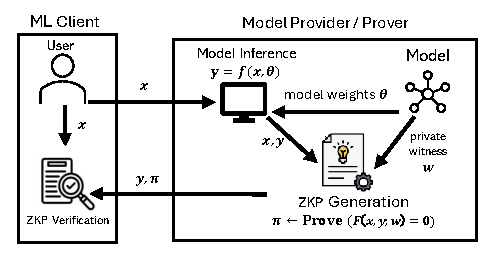
\includegraphics[width=\linewidth]{figures/background/zkInfer_workflow.pdf}
    \caption{
    zkML inference and verification workflow. The model provider acts as the prover, returning an output $y$ and a proof $\pi$ attesting that $y$ was produced by evaluating the claimed model on input $x$.
    }
    \Description{
        Diagram showing a client sending an input to a machine-learning service provider. The provider evaluates a model, generates a zero-knowledge proof of correct inference, and returns the output and proof to the client, which verifies the proof.
    }
    \label{fig:zkml-workflow}
\end{figure}

\subsection{Proof Generation as a Systems Bottleneck}
\label{sec:proving-bottleneck}

The per-request proving path does more than execute the model. Conventional ML runtimes map tensor operations to optimized kernels and reuse memory once intermediate values are no longer live~\cite{chen2018tvm,rotem2018glow}. A zkML prover must additionally encode the computation as arithmetic constraints, construct the corresponding witness, and process the resulting circuit cryptographically~\cite{chen2024zkml}.

These requirements introduce work and state beyond ordinary inference. Operations such as fixed-point arithmetic, comparisons, and nonlinearities may require range checks, lookups, bit decompositions, or auxiliary constraints~\cite{chen2024zkml,kang2024scaling,liu2021zkcnn}, increasing both constraint count and witness size. Proof generation also retains witness assignments together with proving-key data, auxiliary polynomials, and temporary buffers used by the proving system. In Halo2~\cite{halo2}, these structures can drive the working set into the hundreds of gigabytes for large models~\cite{chen2024zkml}.

As a result, zkML proof generation is both compute- and memory-intensive. The added cryptographic work increases request latency, while large per-proof memory footprints constrain model size and limit how many proofs can run concurrently. These costs make proof generation a primary systems bottleneck in zkML serving.

% These costs become especially restrictive when the full model is
% treated as a single proving invocation. The request remains bound to
% one machine for the duration of proof generation, the complete
% working set must fit within that machine's memory capacity, and
% additional prover machines cannot directly accelerate the request.
% The serving system also sees only one long-running, high-memory task,
% limiting its ability to place, schedule, or recover smaller units of
% work independently. The systems bottleneck is therefore not only how
% efficiently model operations are represented within the proof system,
% but also the granularity at which the resulting proving workload is
% executed.

% This observation motivates a different question: must the full model
% be the unit of proof execution? The next section describes how the
% model computation graph exposes smaller units that may provide a
% basis for decomposing proof generation.



\begin{figure}[t]
\centering
\scriptsize
\begin{tikzpicture}[
op/.style={draw, rounded corners, minimum width=0.85cm, minimum height=0.42cm, align=center},
job/.style={draw, dashed, rounded corners, inner sep=4pt},
edge/.style={-{Latex[length=1.5mm]}, thick},
node distance=0.55cm and 0.75cm
]

\node[op] (x) {Input};
\node[op, right=of x] (conv) {Conv};
\node[op, right=of conv] (relu) {ReLU};

\node[op, above right=0.35cm and 0.85cm of relu] (a) {Op};
\node[op, below right=0.35cm and 0.85cm of relu] (b) {Op};

\node[op, right=2.0cm of relu] (add) {Add};
\node[op, right=of add] (y) {Output};

\draw[edge] (x) -- (conv);
\draw[edge] (conv) -- (relu);
\draw[edge] (relu) -- node[above left] {$t_1$} (a);
\draw[edge] (relu) -- node[below left] {$t_1$} (b);
\draw[edge] (a) -- node[above right] {$t_2$} (add);
\draw[edge] (b) -- node[below right] {$t_3$} (add);
\draw[edge] (add) -- (y);

\node[job, fit=(conv)(relu), label=below:{Job 1}] {};
\node[job, fit=(a), label=above:{Job 2}] {};
\node[job, fit=(b), label=below:{Job 3}] {};
\node[job, fit=(add), label=below:{Job 4}] {};

\end{tikzpicture}
\caption{
Example inference graph partitioned into four proving jobs. Dashed regions denote jobs; tensors \(t_1\), \(t_2\), and \(t_3\) cross partition boundaries.
}
\label{fig:prover-job-graph}
\end{figure}


\subsection{Model Computation as a Graph}
\label{sec:model-graph}
Before inference is lowered into constraints, many zkML pipelines represent the model as an ONNX graph, where nodes correspond to tensor operators, such as convolutions, matrix multiplications, activations, and reshaping operations, while edges carry intermediate tensors between operators~\cite{onnx-paper}. Figure~\ref{fig:prover-job-graph} illustrates how this graph can be partitioned into a set of proving jobs. Each job contains one or more operators and proves the corresponding portion of the model computation. When an edge crosses a job boundary, the tensor produced by the upstream job becomes an input to the downstream job. A partition therefore determines both the computation assigned to each proving job and the intermediate tensors that form the interfaces between jobs. Although lowering changes how individual operators are encoded within the proof system, it preserves the underlying data dependencies of the model. The inference graph therefore provides a natural basis for partitioning proof generation into jobs. The next section examines how partition granularity affects prover time, peak memory, job heterogeneity, and the parallelism available to the serving system.



% \subsection{Model Computation as a Graph}
% \label{sec:model-graph}
% Before inference is lowered into constraints, many zkML pipelines represent the model as an ONNX graph, where nodes are tensor operators, such as convolutions, matrix multiplications, activations, and reshaping operations, and edges carry intermediate tensors produced by one operator and consumed by another~\cite{onnx-paper}. Figure~\ref{fig:prover-job-graph} shows how this graph can be partitioned into proving jobs. Each job contains one or more operators and proves only the corresponding part of the model computation. When an edge crosses a job boundary, the intermediate tensor produced by one job must be supplied as an input to the job that consumes it. The graph therefore determines both the computation assigned to each job and the intermediate values that connect the resulting proofs. Lowering the model into constraints changes how each operator is represented inside the proof system, but the same values must still flow between the corresponding parts of the computation. The inference graph therefore provides a natural basis for decomposing proof generation. The next section examines how proving granularity affects prover time, memory use, job heterogeneity, and available parallelism.





% Splitting an ONNX graph is straightforward as a graph operation, but the choice of split has important consequences for proof generation. The graph already specifies operators and tensor dependencies, so a system can form subgraphs by cutting along edges in the dataflow. However, each cut turns an internal tensor into cross-job data, and each subgraph becomes a separate prover invocation with its own time and memory cost. Thus, the challenge is not merely to divide the ONNX graph, but to choose a proving granularity that reduces prover resource requirements without creating excessive coordination overhead or poorly balanced jobs.
